%%%%%%%%%%%%%%%%%%%%%%%%%%%%%%%%%
%   Voreinstellungen  / Präambel:
%%%%%%%%%%%%%%%%%%%%%%%%%%%%%%%%%
\documentclass[11pt,a4paper, onecolumn, twoside]{scrartcl}

\usepackage[latin1]{inputenc}
\usepackage{fancyhdr,amsmath,amsfonts, calc, tabularx, amssymb}
\usepackage{graphicx, float, paralist}	% Bilder einbinden können, die auch gleiten können
\usepackage{makeidx}	% Index erzeugen können
\usepackage[usenames,dvipsnames]{xcolor}	% Farben auch direkt ansteuern können per Name
\usepackage[font={ small}, labelsep=period,format=plain]{caption} % Bildunterschriften

\usepackage[linkbordercolor={1 1 1}, citebordercolor={1 1 1}, pdfborder={1 1 1}, plainpages=false]{hyperref}	% Hyperlinks korrekt einfärben
\usepackage[nottoc]{tocbibind}	% Inhaltsverzeichnistiefe vorgeben können
\usepackage{subfig}	% Subbilder erzeugen können
\usepackage{trsym}	% 
\usepackage{multirow}	% In Tabellen auch Inhalte über mehrere Zeilen definieren können
\usepackage{wrapfig}	% Abbildungen von Text umfließen lassen können
\usepackage{tabularx} % Tolle Tabellen, die automatisch die korrekte Breite haben
\usepackage{textcomp}	% "Mü" auch im normalen Text verwenden können!
\usepackage[]{bookmark}
\usepackage{wasysym, txfonts}	% Mathematische Elementsymbole (Complex, etc.)
%\usepackage{cite} % Zitate auch direkt angeben können, für z.B. [1-4]



% Mögliche Grafikformate, die man einbinden kann. Der Compiler sucht übrigens genau in dieser Reihenfolge,
% falls KEINE Endung im jeweiligen \includegraphics{} verwendet wird!
\DeclareGraphicsExtensions{.png, .jpg, .bmp, .pdf}

% Style-Datei liegt um übergeordneten Verzeichnis. In dieser Datei werden alle Format-relevanten
% Einstellungen vorgenommen. Diese betreffen das komplette Manual und sollten nur mit Bedacht geändert werden!
\usepackage{TexManual}

%Matlab als Kommando anmelden, da es besondere Schreibweisen hat, genauso für PHOTOSS, Condor, etc.
\newcommand{\Matt}{\mbox{MATLAB\textsuperscript{\textregistered}}}
\newcommand{\MattZeile}{\mbox{MATLAB\textregistered}}
\newcommand{\MAT}{\Matt}

\newcommand{\PHO}{\mbox{PHOTOSS}}
\newcommand{\PS}{PScript}
\newcommand{\Condor}{Condor\textsuperscript{\textregistered}}
\newcommand{\CondorZeile}{Condor\textregistered}

% Name der ausführbaren PHOTOSS-EXE-Datei:
\newcommand{\PHOEXE}{\mbox{\lstinline!PHOTOSS.exe! }}
% Bigbreak als verkürztes Kommando:
\newcommand{\bb}{\bigbreak}
% Breite für die PHOTOSS-Parameter-Tabllen in pt als Platzhalter:
\newcommand{\PHOTableWidth}{440pt}

\newcommand{\PQUEUE}{\mbox{PQueue}}
\newcommand{\PJOB}{\mbox{PJob}}
\newcommand{\PJOBCMD}{\mbox{\PJOB Cmd}}

\fancyfoot[LO,RE]{ \textcolor{phocolor}{\emph{PQueue User Manual}}}
\usepackage{tikz}
\usetikzlibrary{snakes}
\usepackage{../PScript}
\usepackage{../PQueueScript}

\definecolor{gray}{gray}{0.9}
\newcommand{\photoss}{\PHO{}}
\newcommand{\pjob}{\PJOB{}}
\newcommand{\matlab}{\Matt{}}
\newcommand{\pho}{.pho}
\newcommand{\pscript}{.pscript}
\newcommand{\pjobeditor}{\mbox{PJobEditor}}
\newcommand{\mac}{\mbox{MacOSX\textsuperscript{\textregistered}}}

% Index (genauer: Stichwortverzeichnis) erstellen:
\makeindex

%%%%%%%%%%%%%%%%%%%%%%%%%%%%%%%%%
%   Eigentliches Dokument beginnen
%%%%%%%%%%%%%%%%%%%%%%%%%%%%%%%%% 
\begin{document}

%%%%%%%%%%%%%%%%%%%%%%%%%%%%%%%%%
%   Titelblatt
%%%%%%%%%%%%%%%%%%%%%%%%%%%%%%%%% 
	\begin{titlepage}

	\vspace*{2cm}

	\begin{center}
		
\includegraphics[width=11.00cm]{../../PQueue/Gui/Resources/splash_gross.png}\\
		\vspace*{3cm}
	 \Huge{  \textcolor{phocolor}{\textbf{User Manual}}}\\
	\end{center}

	\vspace{1cm} 
	\begin{center}
		% TODO: Versionsnummer
	\textcolor{phocolor}{\textbf{\Huge \PQUEUE{} 0.1}}
	\end{center}

	\end{titlepage}

%%%%%%%%%%%%%%%%%%%%%%%%%%%%%%%%%
%   Fancy Page 2 (Jens' Style == Crappy) ;-)
%%%%%%%%%%%%%%%%%%%%%%%%%%%%%%%%% 
\newpage 
\pagestyle{empty}

\vspace*{16.0 cm}
\noindent \Large{Creation Date:}\\
\noindent \Large{\today}\bb

\noindent \Large{\PQUEUE{} manual in \LaTeX{} by: }\\
\noindent \Large{Nicolas Luck}\\
\normalsize

%%%%%%%%%%%%%%%%%%%%%%%%%%%%%%%%%
%   Schriftgröße auf normal zurückstellen:
%%%%%%%%%%%%%%%%%%%%%%%%%%%%%%%%%

%%%%%%%%%%%%%%%%%%%%%%%%%%%%%%%%%
%   Inhaltsverzeichnis:
%%%%%%%%%%%%%%%%%%%%%%%%%%%%%%%%% 
\newpage
\hypertarget{TargetEinsprungspunktHilfe}{}
\tableofcontents
\pagestyle{fancy}
\newpage

%%%%%%%%%%%%%%%%%%%%%%%%%%%%%%%%%
%   Eigentliche Inhalte des Manuals:
%%%%%%%%%%%%%%%%%%%%%%%%%%%%%%%%% 

\section{Introduction} \hypertarget{TargetIntroduction}{}
\newpage
\PQUEUE{} is a software that accompanies \PHO{}.
It's main purpose is to help distributing \PHO{} calculation jobs within a pool of working machines.
Therefore it uses \Condor{} as underlying grid computation framework.\bb

To represent a \PHO{} calculation job, a novel file format called \nameref{section:pjob} is introduced.
\PJOB{} files can be created and edited using the \nameref{section:pjob-editor} which is also distributed together with \PHO{} and \PQUEUE{}.\bb

\PQUEUE{} enables the user to open \PJOB{} files and insert them into a queue - hence it's name.
Jobs are processed according to the sequence in this queue,
and either are executed locally or on a remote machine via \Condor.
In both cases, a job is calculated by running the command line version of \PHO{} on it.\bb

After successfully running the simulation contained in the \PJOB{} file,
\PQUEUE{} reads the \PJOB's results into the applications memory.
Then, after receiving results of multiple job instances, the user may write all results into one single CSV file for example
or visualize this potentially multidimensional data in a three dimensional view within \PQUEUE.\bb

Similar to \PHO{} and PScript, utilizing a ECMAScript engine \PQUEUE{} is also scriptable.
This enables the user to build and update the job queue automatically and with user defined behavior.
Doing long-winded optimizations by calculating further simulation parameters as a function of former results
is the main use case for \PQUEUE{} scripts.\bb



\subsection{Outline}

Because of \PJOB{} and its concepts being a prerequisite for \PQUEUE{},
this manual starts with a detailed description of the \PJOB{} file format in section \ref{section:pjob}.

\PJOB{} files have to be created and edited in order to have jobs \PQUEUE{} can work with.
Section \ref{section:pjob-cmd} covers \nameref{section:pjob-cmd}, a command line tool that does this job.
\nameref{section:pjob-editor} is its GUI equivalent and is described in section \ref{section:pjob-editor}.
For a quick introduction, you could skip the first chapters and start with section \ref{section:pjob-editor}
and learn by example.

Section \ref{section:pqueue} covers \PQUEUE's main use cases. 
\newpage

\section{\PJOB} \hypertarget{TargetPJob}{}
\label{section:pjob}
\newpage
Think of a \PJOB{} file as self contained \PHO{} calculation job.
A \PJOB{} file contains all information needed to run the job.
The only extra part is \PHO{} itself.\bb

This file format was introduced to make the creation and sharing of complex simulation scenarios easier.
A \pjob\ file incorporates all data necessary to run a complex job.
Depending on the actual simulation scenario this may be several \pho\ files, \matlab\ files, \pscript\ files
or some user defined data structures.\bb

\pjob\ files may declare parameters that have to be provided when executing the job.
Also \pjob\ files may have multiple results.
Parameters and results constitute the interface of a concrete \pjob\ file.
Systems such as \PQUEUE{} don't need to know how a \pjob\ is implemented.
The numbers and names of parameters and results is all it needs to know
in order to work with the \pjob{}. 
A \pjob\ file uses XML files to determine what parameters may be provided when executing the job,
what results are created and in which files these results are written. \bb

When running a \pjob\ file \photoss\ writes the simulation results into the executed \pjob\ file.
Already existing results are preserved so a \pjob\ file saves the history of all executions of a job.\bb






\subsection{Creating a \PJOB{} file}
The rest of this section covers the details of the \pjob\ file format.
In order to create a \pjob\ file, you won't need to know all of this if you use the \PJOB-Editor.
See section \ref{section:pjob-editor} for a description of how to create \pjob\ files with the \PJOB-Editor.\bb

If you want to create \pjob\ files programmatically you could either write \pjob\ files yourself
according to the definitions given in this chapter
or you could create all the \pjob file's contents in a separate directory and archive this directory
into a \pjob\ file using the \PJOBCMD\ tool.
See section \ref{section:pjob-cmd} for more information on this.\bb

Either way, you need to know the basics on how to implement a \pjob.
\pjob\ files use \PS{} to enable the user to do user defined actions within an \PJOB{}.
Every \PJOB{} needs to include a main.pscript file that gets executed when \PHO{} runs the job.
In main.pscript, code can be provided that loads and runs a \pho\ file for example.
Before executing the script, \PHO{} changes its current working directory to the resources directory
where the main.pscript file resides.
Also before executing, declared parameters are set to the provided values
(or default values if no values are provided to \PHO{}' command line)
and are made available in the script's context.

For example, if a \PJOB{} file declares a parameter named \textit{length}
and contains a file named \textit{my\_system.pho}
the following main.pscript will run the provided \pho\ file
after setting the value of \textit{length} as the fiber's length:

\lstset{language=JavaScript}
\lstset{backgroundcolor=\color{gray}}
\begin{lstlisting}
sim = Application.openSimulation("my_system.pho");
sim.SMF.length = Application.parameters.length;
sim.run();
\end{lstlisting}

It is the \PJOB{}'s creator's responsibility to assemble a functional \PJOB{} file.
The main.pscript listed above relies on a \textit{my\_system.pho} containing a component named \textit{SMF}
that has a parameter named \textit{length}.
Also it relies on the declaration of a \PJOB{} file parameter named \textit{length}.
If any of these assumptions is not met \PHO{} won't be able to execute and will stop premature
leaving an empty run directory without results.




\subsection{Structure}
\label{pjob:structure}
\pjob\ files are archives containing a particular file structure as depicted in figure \ref{filestructure}.
\begin{figure}[h!]
%\centering
\caption{File structure of a \pjob\ file. \textbf{Bold} entries represent directories.}
\label{filestructure}
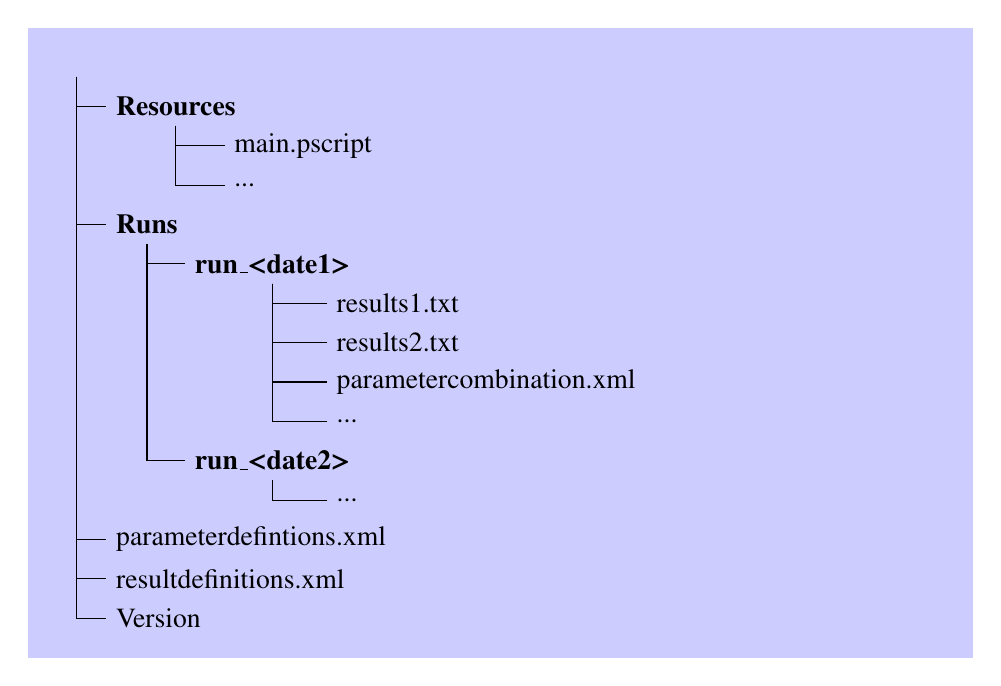
\begin{tikzpicture}
\fill[blue!20] (0,0) rectangle (12cm,-8cm);
\draw (0.5,-0.5) node[anchor=west](root) {\\};
	\draw (1,-1) node[anchor=west,font=\bfseries](Res) {Resources};
		\draw (2.5,-1.5) node[anchor=west](main) {main.pscript};
		\draw (2.5,-2) node[anchor=west] (ResDots){...};
	\draw (1,-2.5) node[anchor=west,font=\bfseries] (Runs) {Runs};
		\draw (2,-3) node[anchor=west,font=\bfseries] (Run1) {run\_\textless date1\textgreater};
			\draw (3.8,-3.5) node[anchor=west](Run1Main) {results1.txt};
			\draw (3.8,-4) node[anchor=west] (Run1Dots) {results2.txt};
			\draw (3.8,-4.5) node[anchor=west](Run1Params) {parametercombination.xml};
			\draw (3.8,-5) node[anchor=west](Run1Results) {...};
		\draw (2,-5.5) node[anchor=west,font=\bfseries] (Run2) {run\_\textless date2\textgreater};
			\draw (3.8,-6) node[anchor=west] (Run2Dots) {...};
	\draw (1,-6.5) node[anchor=west] (Parameterdefinitions) {parameterdefintions.xml};
	\draw (1,-7) node[anchor=west] (Resultdefinitions) {resultdefinitions.xml};
	\draw (1,-7.5) node[anchor=west] (Version) {Version};

\draw (root.south) |- (Res.west);
\draw (root.south) |- (Runs.west);
\draw (root.south) |- (Parameterdefinitions.west);
\draw (root.south) |- (Resultdefinitions.west);
\draw (root.south) |- (Version.west);
\draw (Res.south) |- (main.west);
\draw (Res.south) |- (ResDots.west);
\draw (Runs.south) |- (Run1.west);
\draw (Runs.south) |- (Run2.west);
\draw (Run1.south) |- (Run1Dots.west);
\draw (Run1.south) |- (Run1Main.west);
\draw (Run1.south) |- (Run1Params.west);
\draw (Run1.south) |- (Run1Results.west);
\draw (Run2.south) |- (Run2Dots.west);
\end{tikzpicture}
\end{figure}


The following entries are mandatory:
\begin{itemize}
\item Directory \textit{Resources} containing a file \textit{main.pscript}
\item Directory \textit{Runs} (may be empty)
\item Files \textit{parameterdefintions.xml}, \textit{resultdefinitions.xml} and \textit{Version}
\end{itemize}
The directory \textit{Resources} may contain any number of files or directories of any depth.
\textit{Resources/main.pscript} must be a valid \textsc{PScript} file.
For every (already completed) execution of the job there is a subdirectory in the \textit{Run} directory.
These subdirectories are named \textit{run\_} plus the date of the execution
in the format \textit{YYYYMMDD\_hhmm} (so that lexical sorting makes it easy to find the latest run).

File \textit{Version} contains the \pjob\ file's version as string.
So for the first version this is \textit{``1.0''}. Will be different in future versions of \pjob\ files.

\subsubsection{Underlying archive format}
\label{pjob:archive_format}
\pjob\ files use a self-made binary archive format to concatenate the files contained in a \pjob\ file.
The first 21 bytes are occupied by the file header.
It starts with the 9 byte string \texttt{PJobFile\textbackslash n}
followed by the file's version number represented as a 4 byte little endian integer (TODO: signed or unsigned?).
The header's third and last field is a 8 byte little endian long integer (TODO: signed or unsigned?)
that tells the files last modification date in seconds since the Unix Epoch (00:00:00 UTC on 1 January 1970).

The file's content consists of chunks,
one for every file that is archived in it.
Each chunk itself consists of a chunk header and its content (the file content).
The chunk header's first field is a newline terminated string that represents the filename
associated with this chunk,
including its relative (to this archive), forward slash (\texttt{/})
seperated file path (for example \texttt{Resources/main.pscript}).
The filename is followed by the file's last modification date as a 8 byte little endian long integer,
again representing the number of seconds since the Unix Epoch.
Third and last chunk header field is a 4 byte little endian integer representing
the chunk's body's size in bytes.
This is directly followed by the body that is the file's zlib compressed content.

\begin{figure}[h!]
\caption{\pjob's underlying binary format.}
\label{binary_format}
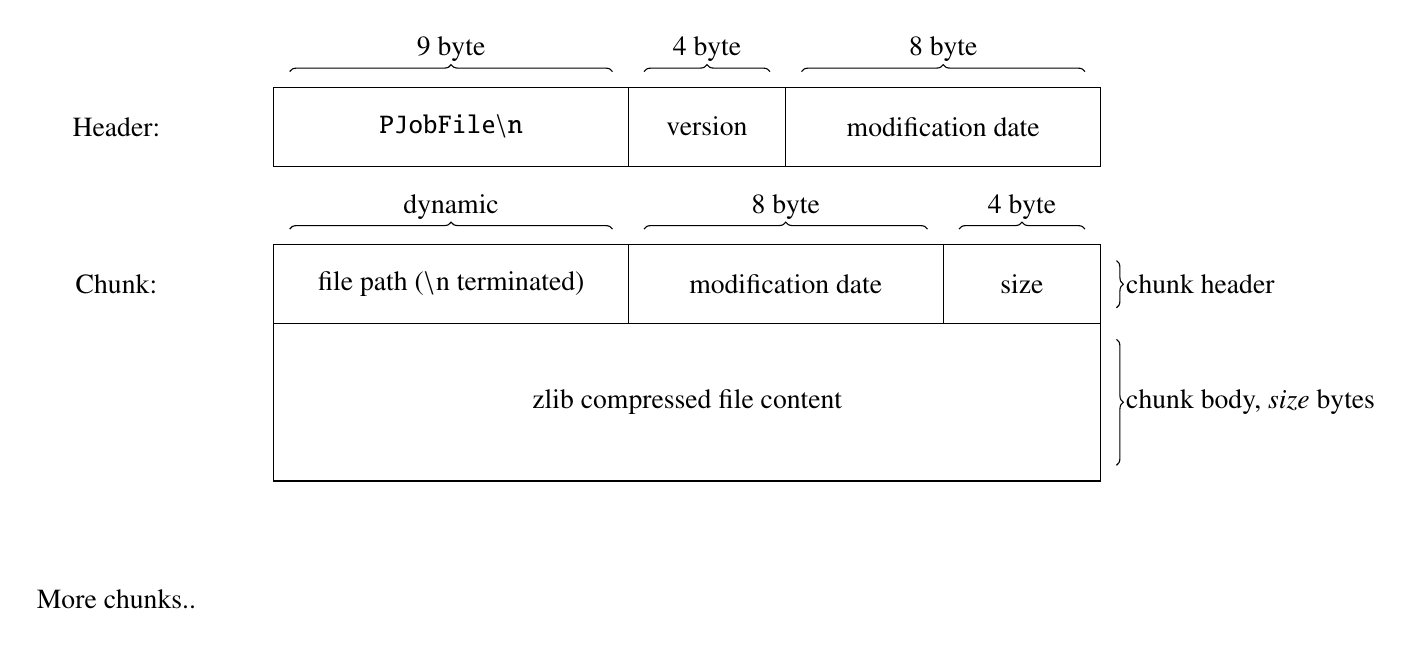
\begin{tikzpicture}
	\draw (-2,-0.5) node {Header:};
	\draw (0,0) rectangle (4.5,-1) rectangle (6.5,0) rectangle (10.5,-1);
	\draw (2.25, -0.5) node {\texttt{PJobFile\textbackslash n}}
	      (5.5, -0.5) node {version}
	      (8.5, -0.5) node {modification date};
	
    \draw[snake=brace] (0.2,0.2) -- node[above]{9 byte} (4.3,0.2)
                       (4.7,0.2) -- node[above]{4 byte} (6.3,0.2)
                       (6.7,0.2) -- node[above]{8 byte} (10.3,0.2);

    \draw (-2,-2.5) node {Chunk:};
    \draw (0,-2) rectangle (4.5,-3) rectangle (8.5,-2) rectangle (10.5,-3) rectangle (0,-5);
	\draw (2.25, -2.5) node {file path (\textbackslash n terminated)}
	      (6.5, -2.5) node {modification date}
	      (9.5, -2.5) node {size}
	      (5.25, -4) node {zlib compressed file content};
	
	\draw[snake=brace] (0.2,-1.8) -- node[above]{dynamic} (4.3,-1.8)
                       (4.7,-1.8) -- node[above]{8 byte} (8.3,-1.8)
                       (8.7,-1.8) -- node[above]{4 byte} (10.3,-1.8)
                       (10.7,-2.2) -- node[right]{chunk header} (10.7,-2.8)
                       (10.7,-3.2) -- node[right]{chunk body, \textit{size} bytes} (10.7,-4.8);

    \draw (-2,-6.5) node {More chunks..};
\end{tikzpicture}
\end{figure}

This format makes it easy to add files to the archive,
chunks can be appended at the end of the file.
There is no sorting required.
The tree-like file structure is implied by the file names which also include the path
and therefore the directory.
One negligible drawback is that there is no way to have an empty directory.
The file's contents can be scanned by hopping from chunk header to chunk header,
omitting the content.

\subsubsection{Parameters}
\label{pjob:parameters}
A \pjob\ file may declare parameters that can be assigned values to when executing the job with \photoss.
Once declared, these parameteres will be available in the main.pscript's context,
that is the \pjob's script may assume that variables with the parameter's names
have been set before executing the main.pscript.
Furthermore the parameter's values are checked to be within the specified boundaries.

The file \textit{parameterdefinitions.xml} defines which parameters may be provided when executing the job.
This must be consistent with the code in \textit{main.pscript},
i.e. parameters needed by the script must be declared here.
For every parameter a name and a default value has to be provided,
a minimum or maximum value can be provided.
A \textit{parameterdefinitions.xml} file may look like this:
\lstset{language=XML}
\lstset{basicstyle=\color{black},backgroundcolor=\color{gray}}
\begin{lstlisting}
<parameterdefinitions>
	<parameter>
		<name>length</name>
		<defaultValue>100</defaultValue>
	</parameter>
	<parameter>
		<name>power</name>
		<unit>dBm</unit>
		<defaultValue>5</defaultValue>
		<min>1</min>
		<max>15</max>
	</parameter>
</parameterdefinitions>
\end{lstlisting}
A XML Schema Definition for this XML file is provided in the appendix.\bb

When executed a \textit{parametercombination.xml} file is saved in the run directory.
This file contains the information for which parameter values the job was executed.
It is either constructed by \photoss\ according to the default values
provided with the \textit{parameterdefinitions.xml}
or it was passed by the user as an argument in order to run the job with parameter values
differing from the default values.

A \textit{parametercombination.xml} may look like this:
\begin{lstlisting}
<parametercombination>
	<parameter>
		<name>length</name>
		<value>50</value>
	</parameter>
	<parameter>
		<name>power</name>
		<variation>
			<min>3</min>
			<max>7</max>
			<step>1</step>
		</variation>
	</parameter>
</parametercombination>
\end{lstlisting}
Again a XML Schema Definition is provided in the appendix.\bb

On execution parameters are made available to the script.
For every parameter defined in \textit{parameterdefinitions.xml}
the global Property
\lstset{language=JavaScript}
\begin{lstlisting}
Application.parameters
\end{lstlisting}
will have a property named as the corresponding parameter.
These properties have subproperties \textit{isVariation()}
and either \textit{value} or \textit{min}, \textit{max}, \textit{step} and \textit{values}.
So a \textit{main.pscript} according to the example stated above may look like this:
\begin{lstlisting}
if(Application.parameters.length.isVariation()){
	for(var i in Application.parameters.length.values)
		...
}else{
	var length = Application.parameters.length.value;
	...
}

if(Application.parameters.power.isVariation()){
	for(var i in Application.parameters.length.values)
		...
}else{
	var power = Application.parameters.power.value;
	...
}
\end{lstlisting}



\subsubsection{Results}
\label{pjob:results}
All files created on execution reside in the run directory.
Which files are created depends on the code contained in the file \textit{Resources/main.pscript}.
In order to be able to access a job's results without having to know its implementation
the file \textit{resultdefinitions.xml} declares which files contain results
and what format they use.
A \textit{resultdefinitions.xml} declaring one result file which contains two results may look like this:
\lstset{language=XML}
\begin{lstlisting}
<resultdefinitions>
	<resultFile>
		<filename>Results.txt</filename>
		<format>CSV</format>
		<result>
			<name>EOP</name>
		</result>
		<result>
			<name>Q</name>
			<unit>dB</unit>
		</result>
	</resultFile>
</resultdefinitions>
\end{lstlisting}
Allowed format types are \textit{SINGLE\_VALUE} and \textit{CSV}.
\textit{SINGLE\_VALUE} is the format used by \PHO\ component results,
that is only one floating point number as text (i.e. multiple characters)
and nothing else.
Decimal point is ``.''

\textit{CSV} is for \textit{comma separated values} (also called \textit{flat files}) and is the format used by \PHO\ for parameter variation results.
These files consist of rows separated by newline characters.
Each row consists of fields separated by tabulator characters.
The first lines constitute a header (marked with ``\%'') stating the columns names.
Some columns represent varied simulation parameters and some simulation results.
This is indicated by the columns name and is context dependent.
There is one row for each regarded parameter combination.



\subsection{Execution of a \pjob\ file}
When running a \pjob\ file \photoss\ first extracts its contents to a temporary directory.
It then creates a new subdirectory under \textit{Runs}
named \textit{run\_} plus the current date and time
and copies all files and directories from \textit{Resources} to that newly created run directory.
\photoss\ changes its current working directory to that run directory and
executes the \textsc{PScript} file \textit{main.pscript}.
As described above parameters are therefore added to the \textsc{PScript} context before evaluating the script.
After the script has finished execution,
\PHO{} compares all files within the run directory with the files in the resource directory and deletes files
that weren't changed during execution in order to prevent redundancy and \PJOB{} files from becoming too big.
Then the temporary directory
(with the newly created run directory and the results therein)
is written back to the \pjob\ file.


\subsubsection{Providing \PJOB\ parameters on execution}
A \PJOB\ file can be executed by calling \PHO\ with the path to the \PJOB\ file as argument.
\lstset{basicstyle=\color{white},backgroundcolor=\color{black}, language=bash}
\begin{lstlisting}
lucksus:~ nico$ PHOTOSS_cmd Desktop/my_first.pjob
\end{lstlisting}
If no parameter values are given, \PHO\ sets the default values stored with the parameter definition.
Parameter values can be provided by using \PHO's command line switch \textit{--param} (short: \textit{-p})
followed by the parameter's name and a value.
\begin{lstlisting}
lucksus:~ nico$ PHOTOSS_cmd Desktop/my_first.pjob --param length 100
\end{lstlisting}
Multiple parameters are set either by using multiple \textit{--param} switches
\begin{lstlisting}
lucksus:~ nico$ PHOTOSS_cmd Desktop/my_first.pjob -p length 100 -p power 5
\end{lstlisting}
or by using the \textit{--parametercombination} (short: \textit{-c}) switch and providing the path to a parameter combination file
as described in \ref{pjob:parameters} above.
\begin{lstlisting}
lucksus:~ nico$ PHOTOSS_cmd Desktop/my_first.pjob -c Desktop/parametercombination.xml
\end{lstlisting}

\subsubsection{Parameter variations}
\PJOB\ parameters can be set to be varied.
The \PJOB's main.pscript needs to support this, i.e. has to include code that iterates over all variation values, as is shown in \ref{pjob:parameters}.
Variation values can again either be provided via command line, using \PHO's \textit{--param} switch with the syntax described in the \PHO\ application manual
\begin{lstlisting}
lucksus:~ nico$ PHOTOSS_cmd Desktop/my_first.pjob -p length 10:20:1 -p power 5
\end{lstlisting}
or by writing a parameter combination file.
One equivalent to the example above looks like this:
\lstset{language=XML}
\lstset{basicstyle=\color{black},backgroundcolor=\color{gray}}
\begin{lstlisting}
<parametercombination>
	<parameter>
		<name>length</name>
		<variation>
			<min>10</min>
			<max>20</max>
			<step>1</step>
		</variation>
	</parameter>
	<parameter>
		<name>power</name>
		<value>5</value>
	</parameter>
</parametercombination>
\end{lstlisting}


\newpage

\section{\PJOBCMD} \hypertarget{TargetPJobCmd}{}
\newpage
\label{section:pjob-cmd}
\PJOBCMD\ is a command line tool for creating, manipulating and extracting \PJOB\ archive files.
It implements the format specification described in section \ref{pjob:archive_format} (\nameref{pjob:archive_format}).
It is possible to create a valid \PJOB{} file by creating all the necessary files in one directory
and adding that directory to a new \PJOB{} file with this tool.

\subsection{Example usage}
Suppose you have a directory \textit{My\_PJob} with contents according to the \PJOB{} format specification
(see section \ref{pjob:structure} \nameref{pjob:structure}).
\lstset{basicstyle=\color{white},backgroundcolor=\color{black}, language=bash}
\begin{lstlisting}
lucksus:~ nico$ ls
My_PJob

lucksus:~ nico$ ls My_PJob/
Resources
Version
parameterdefintions.xml
resultdefintions.xml

lucksus:~ nico$ ls My_PJob/Resources/
main.pscript
my_system.pho
\end{lstlisting}
You can create a \PJOB{} archive by using the \textit{--create} command line switch:
\begin{lstlisting}
lucksus:~ nico$ PJobCmdLine --verbose --create My_PJob/ --file my.pjob

Opening my.pjob was succesful.

Creating file my.pjob containing:
parameterdefintions.xml
resultdefintions.xml
Version
Resources/main.pscript
Resources/my_system.pho

lucksus:~ nico$ 
\end{lstlisting}\bb

If you want to extract the results after the \PJOB{} was executed
you could either extract all files with \textit{-x} or \textit{--extract},
or you could use \textit{--peek} (\textit{-p}) to extract the result files only.
\begin{lstlisting}
lucksus:~ nico$ PJobCmdLine -v -p Runs/run_20110322_1748 -f my.pjob -o my_results/

Opening my.pjob was succesful.

Extracting files:
/Users/nico/my_results/EyeOpeningPenalty.txt
/Users/nico/my_results/my_system.log
/Users/nico/my_results/parametercombination.xml

lucksus:~ nico$
\end{lstlisting}



\subsection{Command line parameters}
\PJOBCMD\ is controlled via multiple command line switches.
Every switch has a long version that has to be prefixed by two dashes (i.e. \textit{--help})
and an optional short, one character version that has to be prefixed by one dash (i.e. \textit{-h}).
The following list shows all command line parameters with their long version and their optional short version
separated by comma.
Parameters that require arguments, like \textit{--create} or \textit{--file} for example,
need these arguments to be the next following string.
The same list is printed by \PJOBCMD\ when called with the \textit{help} switch.
\begin{itemize}
	\item \textbf{about,?} shows the about page
	\item \textbf{add,a} adds a folder or directory to the specified file and flush() is called
	\item \textbf{create,c} creates a new .pjob-file which ONLY contains the specified folder. Only takes effect if the file is empty,
							doesn't exist or --force is used
	\item \textbf{detail,d} shows a detailed description of the specified command with examples if provided
	\item \textbf{extract,x} extracts all files
	\item \textbf{file,f} specifies the path of the .pjob-file. If it doesn't exist, an empty file will be created automatically					
	\item \textbf{force} sets overwrite-flag for all commands
	\item \textbf{help,h} produces help message
	\item \textbf{out,o} sets the target directory for --extract and --peek
	\item \textbf{peek,p} extracts the specified source files to --out path
	\item \textbf{verbose,v} displays detailed information about the tasks being made, e.g. list of extracted files
\end{itemize}

\newpage

\section{\PJOB-Editor} \hypertarget{TargetPJobEditor}{}
\label{section:pjob-editor}
\newpage
The encouraged way to create and edit \PJOB{} files is to use the \pjobeditor\
that is distributed alongside \PHO\ and \PQUEUE.
This section shows how to use this software by presenting a walkthrough for a simple example.


\subsection{Creating a \PJOB\ file}
Using \pjobeditor, creating a valid \PJOB\ file is as easy as issuing the command \textit{File} -\textgreater \textit{New...}
via the application menu or via the shortcut \textbf{CTRL + N} (\textbf{CMD + N} on \mac).
\pjobeditor\ then prompts for the name of the file to be created.
After creating, the file is automatically opened and presented in \pjobeditor's main window
as depicted in figure \ref{editor:new_job_created}.

\begin{figure}[h!]
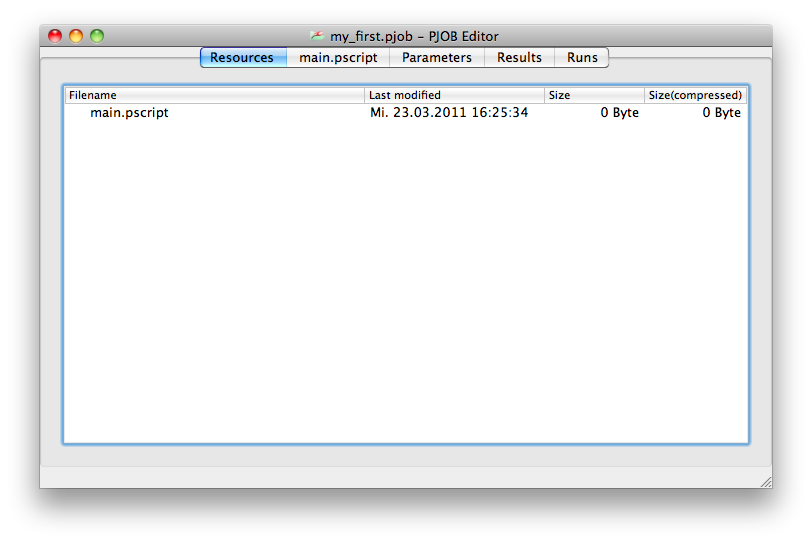
\includegraphics[width=\textwidth]{Screenshots/PJobEditor/new_job_created.png}
\caption{\pjobeditor\ after creating new \PJOB\ file.}
\label{editor:new_job_created}
\end{figure}

It shows multiple tabs from which the \textit{Resource} tab is active.
The resource tab displays the contents of the \PJOB\ file's resource directory
(see section \ref{pjob:structure} \nameref{pjob:structure}) in a tree view.
For a newly created \PJOB\ file, there is only an empty file named \textit{main.pscript}
which is the starting point for the execution of every \PJOB\ file.



\subsection{Adding resources}
By dragging files into this tree view or via the right click context menu,
it is possible to add any number of files or directories to the opened \PJOB\ file.
In order to further describe \pjobeditor's features by example,
suppose we added a directory by right clicking the resources view and choosing \textbf{Make directory},
then renamed that directory to \textit{'PHOs'} by double clicking
and finally added a file called \textit{'my\_system.pho'} to this directory by right clicking the directory
and choosing \textbf{Add resources...} from the context menu
(see figure \ref{editor:pho_added}).

\begin{figure}[h!]
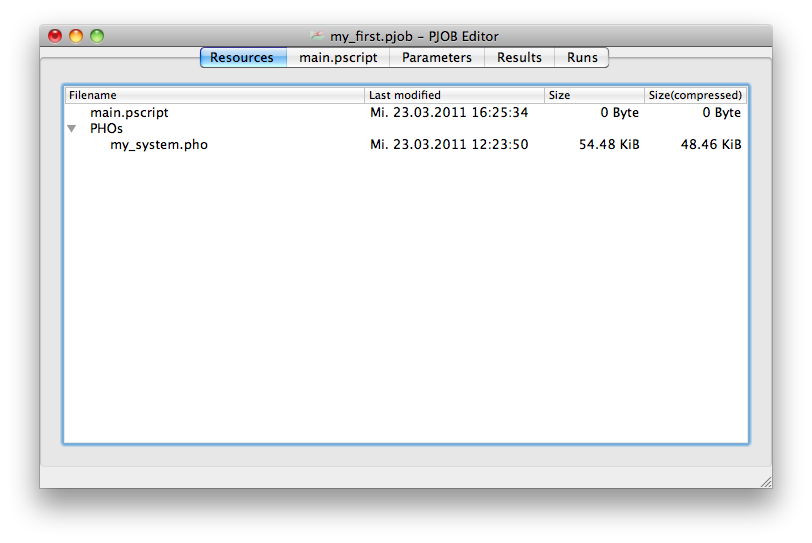
\includegraphics[width=\textwidth]{Screenshots/PJobEditor/pho_added.png}
\caption{\pjobeditor\ after adding a resource file.}
\label{editor:pho_added}
\end{figure}



\subsection{Editing main.pscript}
If we want our \PJOB\ file to actually do something
we have to fill \textit{main.pscript} with \PS\ code.
The simplest example would be to load and run the attached \pho\ file \textit{PHOs/my\_system.pho}.
\PS\ code that accomplishes this would be\footnote{If you are unfamiliar with \PS\
please have a look at the \PS\ manual that is included in this distribution
or see the \PS\ examples which are accessible from \PHO's \PS\ console.}:
\lstset{language=JavaScript, backgroundcolor=\color{gray}, basicstyle=\color{black}}
\begin{lstlisting}
var simulation = Application.openSimulation("PHOs/my_system.pho");
simulation.run();
\end{lstlisting}

It would be possible to write this code into a file in filesystem, rename it to \textit{main.pscript}
and drag it into the \PJOB's resources view, overwriting the empty main.pscript file.
Since editing the \PJOB's behavior is a main use case,
\pjobeditor\ provides support for this task.
\begin{figure}[h!]
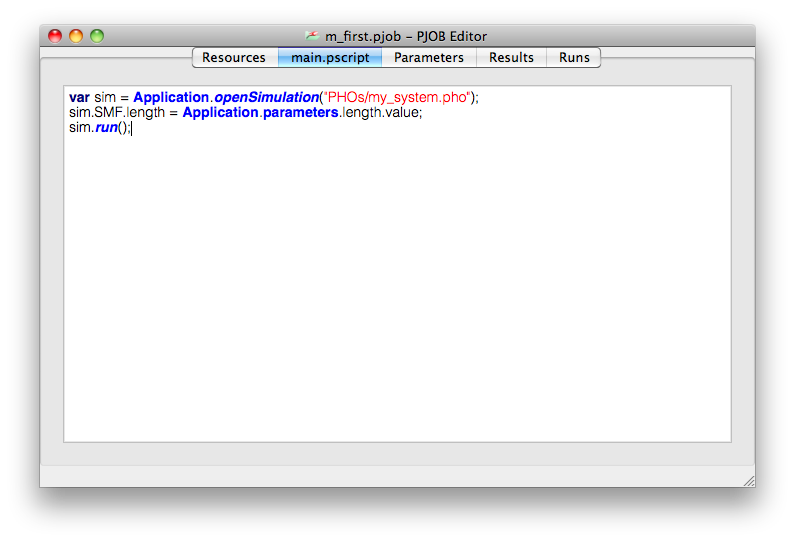
\includegraphics[width=\textwidth]{Screenshots/PJobEditor/main_pscript.png}
\caption{\pjobeditor's main.pscript editor.}
\label{editor:main_pscript}
\end{figure}
Figure \ref{editor:main_pscript} shows the second tab which displays the contents of the \PJOB's main.pscript file
and provides means of editing this file.\bb

Using \PJOB\ files in the context of \PQUEUE,
we would like to parameterize jobs
enabling \PQUEUE\ to distribute calculations of different parameter combinations within the computing grid.
The screenshot shows one additional line:
\begin{lstlisting}
simulation.SMF.length = Application.parameters.length.value;
\end{lstlisting}
This is the \textit{glue code} that takes the \PJOB\ parameter and applies it to the \PJOB's internal structure.
This line implies three facts.
First, there has to be a component named \textit{SMF} within the main network stored in \textit{PHOs/my\_system.pho}.
Furthermore this component needs to have a parameter \textit{length},
what would be expected if this component is of type \textit{Single Mode Fiber}.
Third, the \PJOB file has to declare a parameter named \textit{length}
in order to make \PHO\ add the field \textit{length} to the object \textit{Application.parameters}
when constructing and initializing the script engine that will run this script on execution.
Editing a \PJOB\ file's parameter definitions is also done with \pjobeditor.




\subsection{Editing parameter defintions}
Every parameter of a \PJOB\ has to be declared in order to let \PQUEUE\ know which parameters can be set
and also to make \PHO\ add them to the script context on execution.
As described in section \ref{pjob:parameters},
parameter definitions are stored in an XML file inside the \PJOB\ archive.
You won't have to edit these files manually,
instead \pjobeditor\ provides a GUI editor for parameter definitions within its third tab.
\begin{figure}[h!]
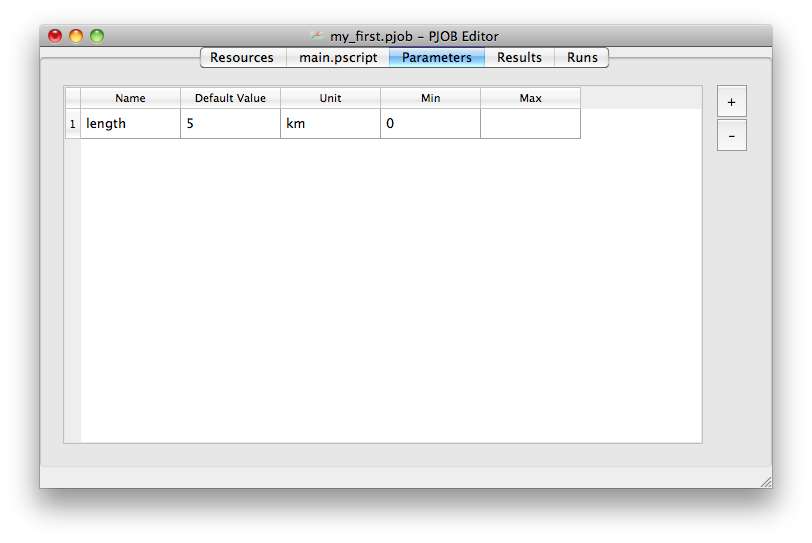
\includegraphics[width=\textwidth]{Screenshots/PJobEditor/parameter.png}
\caption{\pjobeditor's parameter definition editor.}
\label{editor:parameter}
\end{figure}
A new parameter definition is added by clicking the \textit{+} button.
Name, default value and all other properties can be edited by just clicking the appropriate field.
The default value is used by \PHO\ if no value was provided on execution.
\PHO\ makes sure that the \PJOB\ is never executed with parameter values not adhering to the limits set as minimum and maximum value.
Clicking the \textit{-} button removes the selected parameter definition.




\subsection{Editing result definitions}
Depending on the simulation logic implemented in a \PJOB\ file,
results are written to different files and also in different file formats.
In order to let \PQUEUE\ know which file to read results from,
this information has to be stored inside the the \PJOB\ file.
Editing result definitions can be done with \pjobeditor's fourth tab named \textit{Results}.\bb

First, a \textit{result file} has to be added by clicking the \textit{+ result file} button.
Its name has to be changed to the file that is created by \PHO\ or attached scripts on execution.
This has to be a file path relative to the file main.pscript.
Figure \ref{editor:results} shows an example.

\begin{figure}[h!]
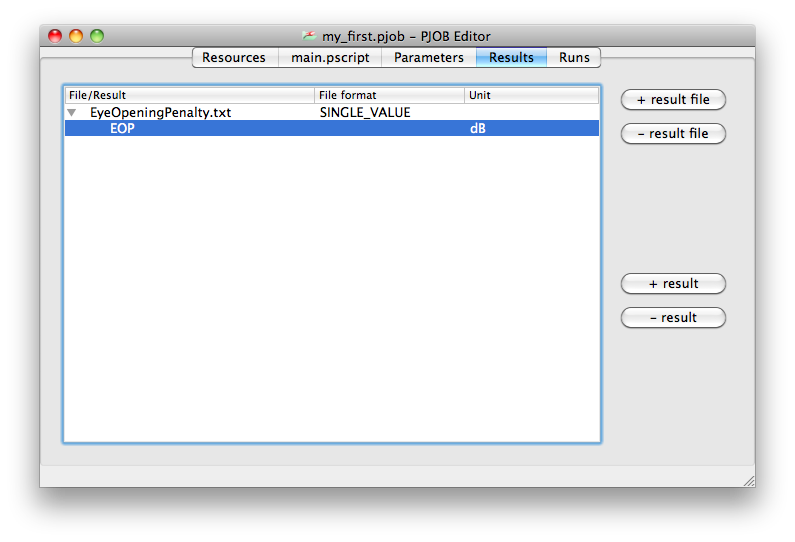
\includegraphics[width=\textwidth]{Screenshots/PJobEditor/results.png}
\caption{\pjobeditor's result definitions editor.}
\label{editor:results}
\end{figure}

The file's format can be set to either \textit{SINGLE\_VALUE} or \textit{CSV}.
For a detailed description on result file formats see section \ref{pjob:results}.
In this case, the result is an ordinary \PHO\ result that is created by the \PHO\ component \textit{Eye Analyzer}.
So this file will contain a single floating point number in text format after execution.
This is exactly what \textit{SINGLE\_VALUE} means.

Only stating the result file's name and format does not suffice.
In case of a \textit{CSV} file, one result file could contain multiple results (and also for multiple parameter combinations).
That is why we have to add a result definition to this result file definition
by clicking the \textit{+ result} button while the result file is selected.
The view now shows an item as the result file's child item.
In case of a \textit{SINGLE\_VALUE} result file,
the name of the result is arbitrary,
but is the name that is used as the result's name within \PQUEUE.
The result's unit can be set by editing the view's third column.
Figure \ref{editor:results_csv} shows an example for a \textit{CSV} result file
as it would be created by \PHO\ when running a parameter variation.
Note that in this case it is mandatory to use the results' names as they are
found in the \textit{CSV} file'as header, i.e. the result names provided by \PHO's components.

\begin{figure}[h!]
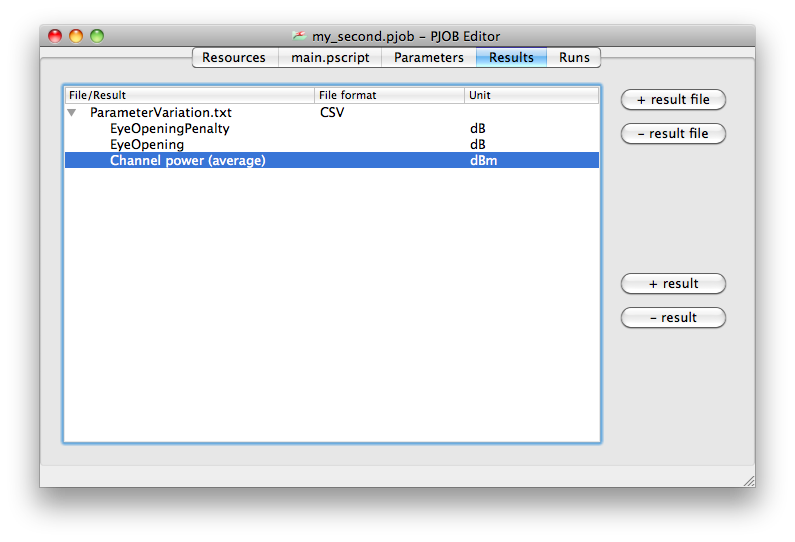
\includegraphics[width=\textwidth]{Screenshots/PJobEditor/results_csv.png}
\caption{\pjobeditor's result definitions for a \textit{CSV} result file.}
\label{editor:results_csv}
\end{figure}




\subsection{Accessing result files}
When executing a \PJOB\ file, \PHO\ adds all created files to a newly created run directory inside the \PJOB\ file.
\pjobeditor\ displays all run directories in it's tree view on tab \textit{Runs}.
Files and folders can be extracted by either dragging them out of this tree view onto the desktop or any other directory
or by right clicking and choosing \textbf{Extract...}.



\newpage

\section{\PQUEUE} \hypertarget{TargetPQueue}{}
\label{section:pqueue}
\setcounter{figure}{0}
\newpage
\subsection{User interface overview}
	When started, \PQUEUE\ shows its main window
	as depicted in figure \ref{pqueue:main_window}.

	\begin{figure}[!ht]
	\centering
	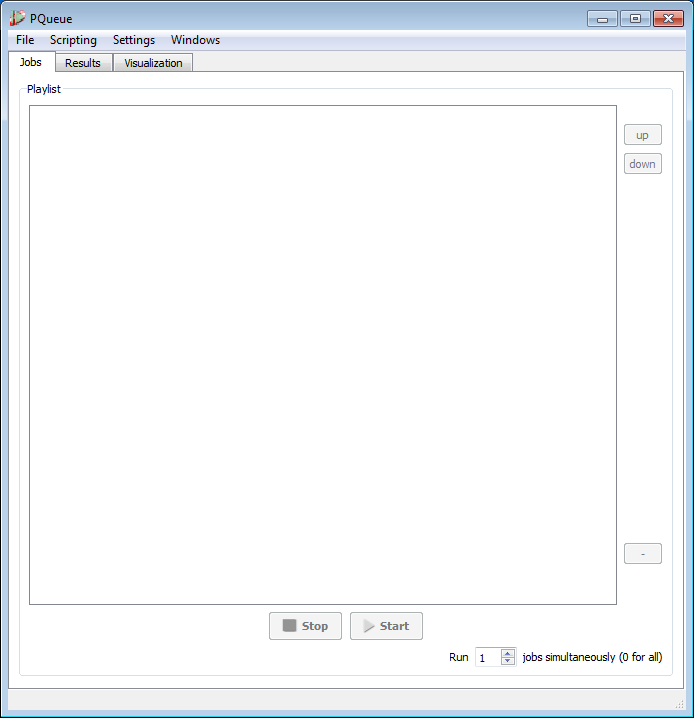
\includegraphics[width=0.75\textwidth]{Screenshots/PQueue/main_window.png}
	\caption{\PQUEUE's main window.}
	\label{pqueue:main_window}
	\end{figure}

	It consists of three tabs, named \textit{Jobs}, \textit{Results} and \textit{Visualization},
	from which the first is displayed in the screenshot.
	Each tab is discussed in detail in the sections \ref{pqueue:running_jobs} (\nameref{pqueue:running_jobs}),
	\ref{pqueue:results} (\nameref{pqueue:results}) and
	\ref{pqueue:visualization} (\nameref{pqueue:visualization}) respectively.

	There are several additional docking windows that are accessible through the application's menu \textbf{Windows}.
	These windows may be moved, resized and docked to any of the main window's edge
	or even detached from the main window.
	Figure \ref{pqueue:all_dock_widgets} shows an example.

	\begin{figure}[!ht]
	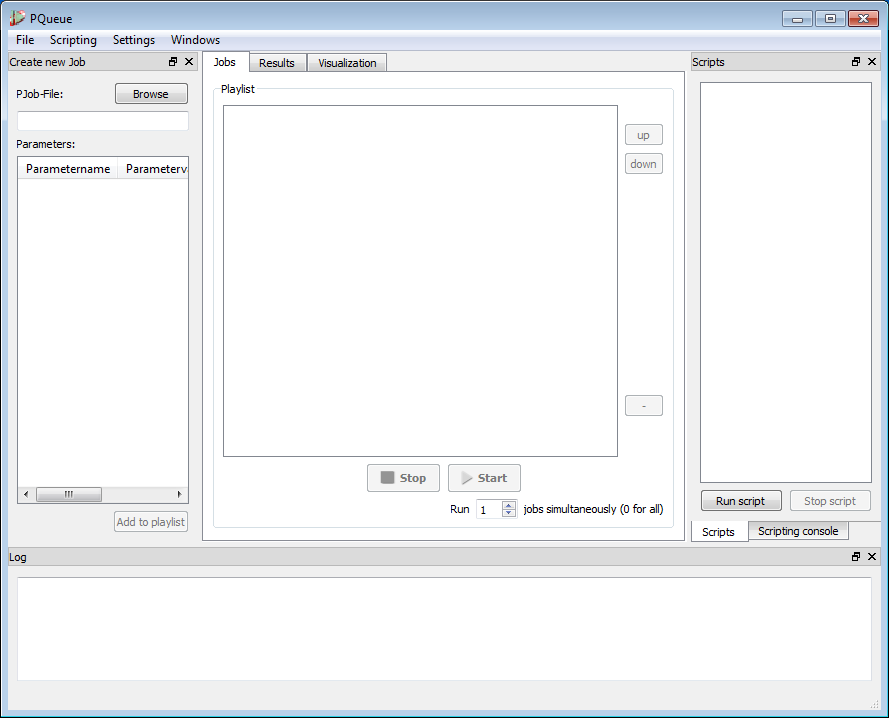
\includegraphics[width=\textwidth]{Screenshots/PQueue/all_dock_widgets.png}
	\caption{All of \PQUEUE's dock windows.}
	\label{pqueue:all_dock_widgets}
	\end{figure}

	The \textit{log} window displays a log showing all \PQUEUE\ events.
	The \textit{create job} window is used to add a job to the playlist by stating a \PJOB\ file
	and providing parameters.
	The \textit{scripting console} window allows the execution of single statements within \PQUEUE's
	script engine and shows script output and results.
	Whole script files are managed and run via the \textit{scripts} window.


\subsection{Settings}
\label{pqueue:settings}

	Also, there is a \textit{settings} window,
	which is accessible via \textbf{Settings} -\textgreater \textbf{Edit...} within the applications main menu.

	\begin{figure}[!ht]
	\centering
	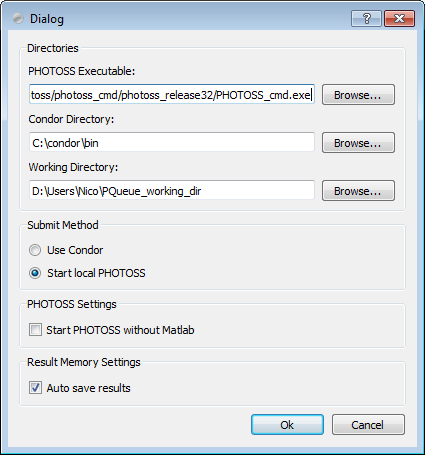
\includegraphics[width=0.6\textwidth]{Screenshots/PQueue/settings.png}
	\caption{\PQUEUE's settings windows.}
	\label{pqueue:settings_window}
	\end{figure}
	
	In order to be able to utilize \PHO\ and \Condor,
	\PQUEUE\ needs to know the directories where these applications are installed in.
	For \PHO\ this should be the directory where the file \textit{PHOTOSS\_cmd.exe} resides.
	For \Condor\ it's the directory containing \Condor's binaries, for example \textit{condor\_submit.exe}.
	
	When running a job,
	\PQUEUE\ creates a temporary directory in which a temporary copy of the \PJOB\ file
	and the \Condor\ log files are stored.
	These directories are created in \PQUEUE's \textit{working directory}
	which is set via the setting's dialog third text field.
	
	Wether to execute a job locally, i.e. on the same machine \PQUEUE\ is running on,
	or to use \Condor\ (i.e. \textit{condor\_submit}) to submit jobs to the \Condor\ pool,
	is set with the \textit{submit method} setting.
	
	If you are using \Condor\ and your pool is heterogenous in terms of \MAT\ installations,
	i.e. you can't assume to have a working \MAT\ installation on every machine,
	you may run into problems if \PHO\ is trying to initialize \MAT\ from the context of a \Condor\ job.
	Therefore \PHO\ provides the command line switch \textit{--matlab} to set a specific \MAT\ version
	or to deactivate \MAT\ support altogether.
	To make \PQUEUE\ start \PHO\ without \MAT\ support,
	activate the setting \textit{Start PHOTOSS without Matlab}.





\subsection{Adding and running jobs}
\label{pqueue:running_jobs}

Within the context of \PQUEUE,
a \textit{job} is a \PJOB\ file \textbf{and} values for all of the file's parameters.
So, in order to add a job to the queue,
you have to choose an already existing \PJOB\ file and provide values for it's parameters.
This is done via the \textit{create job} window as shown in figure \ref{pqueue:adding_jobs}.

\begin{figure}[!ht]
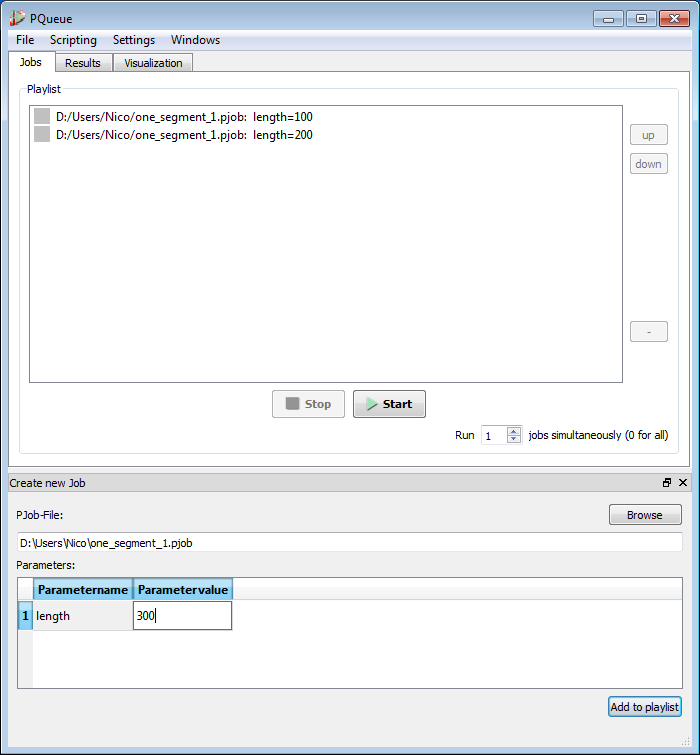
\includegraphics[width=\textwidth]{Screenshots/PQueue/adding_jobs.png}
\caption{Adding jobs to the queue.}
\label{pqueue:adding_jobs}
\end{figure}

As soon as a path to a valid \PJOB\ file is given,
its parameters are read and shown in the table view below.
The values in the column \textit{Parametervalue} can be edited after double clicking.
Pressing the \textit{Add to playlist} button adds the \PJOB\ to the queue with the parameter values currently set in the table view.\bb


Jobs can be arranged within the queue by using the \textit{up} and \textit{down} buttons after selecting a job.
The \textit{-} button removes the selected jobs from the queue.
When \textit{Start} is pressed (or a script triggers execution),
jobs are processed sequentially from top to bottom.
In order to utilize the resources at hand
but avoid overhead,
you might want \PQUEUE\ to execute as many jobs in parallel as there are cores on your machine,
or in the pool respectively.
Therefore the number of jobs executed simultaneously can be set with the spin box in the lower right corner.

\subsubsection{Job states}

During execution, jobs change their state from \textit{queued} over \textit{submitted} and \textit{running}
to \textit{finished} ultimately.
The colored square to the left of the job's file path represents the state.
Gray is for \textit{queued} which means the job is added to the queue but execution was not triggered yet.
Yellow (\textit{submitted}) means the job was submitted to the \Condor\ pool
but no machine was matched yet.
(When executing locally, this state is omitted.)
Dark green means the job is \textit{running} at the moment.
When it's \textit{finished} the square's color changes to light green.





\subsection{Results}
\label{pqueue:results}

Automatically running multiple jobs in sequence
would not make sense if the jobs did not produce results
and also if these results were not collected and saved by \PQUEUE.
Therefore \PQUEUE\ incorporates a result memory
which, in essence, holds a mapping from parameter values to result values
for every \PJOB\ file that was executed.

\begin{figure}[!ht]
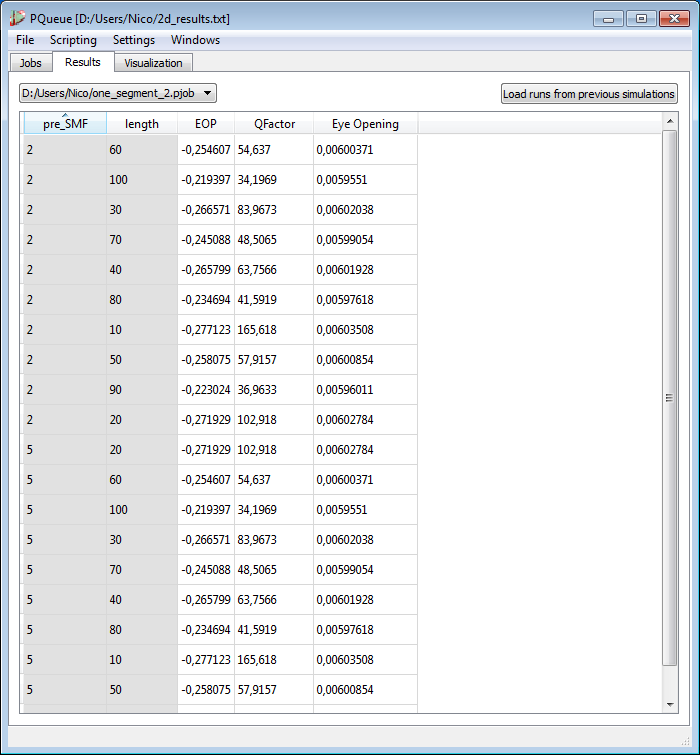
\includegraphics[width=\textwidth]{Screenshots/PQueue/results.png}
\caption{\PQUEUE's result view.}
\label{pqueue:results}
\end{figure}

The main window's second tab shows the result memory by utilizing a table view.
Results are viewed by \PJOB\ file.
That means, first you have to choose the \PJOB\ file for which to view results
by using the combo box in the top left corner.
Now the table view below shows all calculated parameter combinations with their according results
for the selected \PJOB\ file.
Parameter columns are marked gray.
Lines can be sorted by clicking on any column's header.

\subsubsection{Loading and Saving results}
After launching \PQUEUE, its result memory is empty.
When executing jobs,
\PQUEUE\ automatically reads new results from the \PJOB\ file into the result memory.
You might want to save results to a file for further processing.
(Although all results are already saved within the \PJOB\ file's run directories.)
\PQUEUE\ writes and reads its result memory to CSV \footnote{\textit{comma separated values}, also called \textit{flat file}} files.
Writing is triggered via \textbf{File} -\textgreater \textbf{Save results} or \textbf{File} -\textgreater \textbf{Save results as...} and choosing a file path.
The created file contains all information stored in the result memory,
so that \PQUEUE\ is able to restore its result memory by importing a formerly exported file
(via \textbf{File} -\textgreater \textbf{Load results...}).

As mentioned above,
\PJOB\ files contain run directories for every execution.
Since the parameter combination is stored within the run directory,
there already is a result memory in every \PJOB\ file.
Via \textbf{File} -\textgreater \textbf{Import from PJob...},
\PQUEUE\ is able to import all results stored in a \PJOB\ file

If the setting \textit{Auto save results} is activated,
\PQUEUE\ will save the result memory every time new results are received.
For this to work, results must have been saved once before or loaded from file,
so that \PQUEUE\ knows which file to write to.


\subsubsection{Result memory file format}
Exported result memory files can be used to process results with 3rd party tools like Excel for example.
These files store one parameter combination per line with parameter and result values separated by tabulators (\textit{\textbackslash t}).

The first lines, beginning with \textit{\%}, are header files conveying additional information.
For a result space containing results for \textit{n} different \PJOB\ files,
there are \textit{n+1} header lines,
one for each \PJOB\ file and one line (the last header line) stating the column's names separated by tabulators.

The \textit{n} \PJOB\ file header lines contain the \PJOB\ file's path,
its parameter list and its result list.
Parameters are separated from results by two tabulators
to make it possible to distinguish parameters and results without having to know the \PJOB\ file. 



\subsection{Result visualization}
\label{pqueue:visualization}

As long as only one parameter is varied,
the result table described above may be sufficient to view the results.
Since \PQUEUE\ enables the \PHO\ user to conduct huge parameter variations,
possibly variating a huge number of parameters,
it also provides means of visualizing and exploring multidimensional result spaces.

\begin{figure}[!ht]
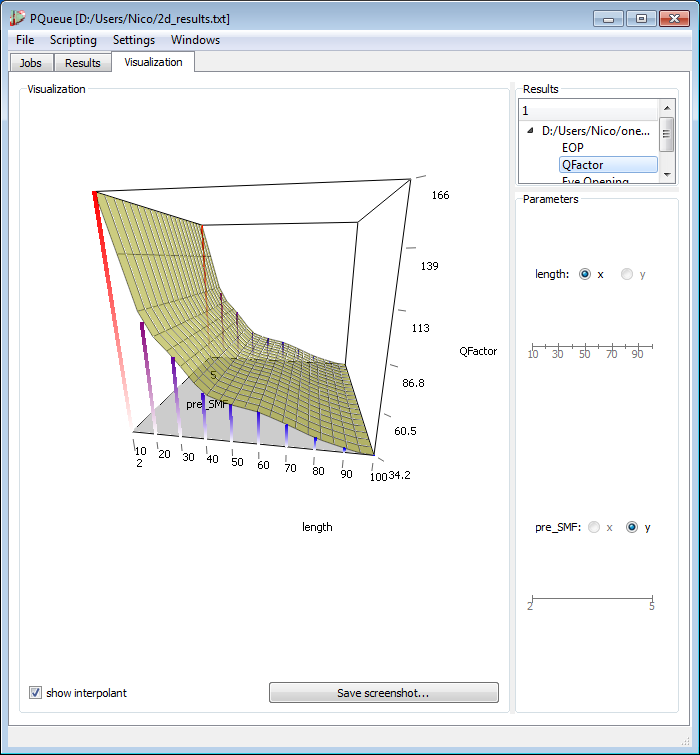
\includegraphics[width=\textwidth]{Screenshots/PQueue/visualization.png}
\caption{\PQUEUE's result visualization.}
\label{pqueue:visualization_screenshot}
\end{figure}

The main window's third tab shows a 3D view visualizing data stored in the result memory.
On the top right, there is a tree view showing all results sorted by \PJOB\ files.
Selecting a result in this tree view determines which result is visualized within the 3D area.
Below the results tree view are radio buttons and sliders for each of the selected \PJOB\ file's parameters.


\subsubsection{3D view}
The 3D view always shows a box for guidance.
When a result is selected in the results tree view,
it also shows the stored values of this result.
Every result value is represented by a colored pillar.
Both color and height correspond to the result's value.
Position of the pillar corresponds to the parameter combination for which
this result value was calculated.
If there are only two parameters this seems natural.
For more parameters,
two have to be chosen to represent the dimensions constituting the box's floor.
The 3D view then shows a two-dimensional intersection of the multidimensional result space.
(See section \nameref{pqueue:vis:parameter} below.)\bb

The view's angle and zoom can be changed by mouse interaction.
Moving the mouse cursor over the 3D view while holding any mouse button down
changes the views angle of sight.
Using the mouse wheel while the mouse cursor is over the view changes the zoom factor.\bb

The view can be saved to an image file (BMP or PNG) by clicking the \textit{Save screenshot...} button
and providing a file path to save to.

\subsubsection{Interpolation function}
\label{pqueue:interpolation_function}
For conveniently exploring a sparse sampled result space,
a multidimensional interpolation function was implemented
that can be added to the 3D view by activating the checkbox \textit{show interpolation function} below the view.

The interpolation method used here is the \textit{Hardy Multi Quadric} which is a \textit{scattered data} interpolation function.
The function is defined by
\textbf{\begin{equation}
	f(x)= \sum_{i=1}^{N} \alpha_{i} R(d_{i}(x)),
\end{equation}}
with $\alpha_{i}$ being the interpolation coefficients that have to be determined
depending on the known data vectors and
$d_i(x)$ being the distance to the $i$-th data vector.
$R(r_i)$ is defined as follows:
\begin{equation}
	R(r_{i}) = (r_{i}^{2} + R_{i}^{2})^{\frac{\mu_{i}}{2}},
	\;
	\mu \neq 0,
\end{equation}
We set $\mu_i = 0.5$ and $R_{i}=0$ for all $i$, simplifying the interpolation function to
\textbf{\begin{equation}
	f(x)= \sum_{i=1}^{N} \alpha_{i} \sqrt{d_{i}(x)}.
\end{equation}}
$\alpha$-coefficients are determined by solving
\begin{equation}
	\min_{\vec{\alpha}} \left\|
	\left( 
	\begin {array} {cccc}
	R(d_{1}(x_{1})) & R(d_{2}(x_{1})) & \dots & R(d_{n}(x_{1})) \\
	R(d_{1}(x_{2})) & R(d_{2}(x_{2})) & \dots & R(d_{n}(x_{2})) \\
	\vdots & \vdots & \vdots & \vdots \\
	R(d_{1}(x_{n})) & R(d_{2}(x_{n})) & \dots & R(d_{n}(x_{n})) \\
	\end {array}
	\right)
	\left( 
	\begin {array} {c}
	\alpha_{1} \\
	\alpha_{2} \\
	\vdots \\
	\alpha_{n}
	\end {array}
	\right)
	-
	\left( 
	\begin {array} {c}
	f_{1} \\
	f_{2} \\
	\vdots \\
	f_{n}
	\end {array}
	\right)
	\right\|.
\end{equation}



\subsubsection{Parameters}
\label{pqueue:vis:parameter}
On the right side of the \textit{Visualization} tab, below the results tree view,
is a list of the selected \PJOB\ file's parameters.
For every parameter, there are two radio buttons reading \textit{x} and \textit{y} respectively
and a slider below.
These widgets control which part of the multidimensional result space is shown within the 3D view.

By clicking the appropriate radio buttons,
one parameter is set to constitute the \textit{x}-axis and another to constitute the \textit{y}-axis.
For these two parameters, the sliders are disabled, because all of their parameter values are shown.
For the remaining parameters, a distinct value has to be set for which to show the results.
This is done by setting the remaining sliders to the appropriate values.
Every parameter combination (i.e. combination of slider positions) will show a different part of the result space.





\subsection{PQueue scripts}
Much like \PHO, \PQUEUE\ incorporates a script engine and therefore can be controlled programmatically.
Jobs can be submitted and results can be evaluated from within a script.
Basically, everything the user could do manually can be done with a script, and even more.
One particular use case for this is the optimization of \PHO\ simulations.
With \PQUEUE\ scripts, parameter combinations that are to be calculated next
can be chosen depending on newly received results.
The section \textit{\nameref{pqueue:scripts:built-in}} below discusses this topic and shows an example.
But first, section \textit{\nameref{pqueue:scripts:executing}} shows how to load and run scripts
and section \textit{\nameref{pqueue:scripts:tutorial}} introduces \PQUEUE\ scripts thoroughly.

\subsubsection{Executing scripts}
\label{pqueue:scripts:executing}
The easiest way to execute script code is by using the script console (\textbf{Windows} -\textgreater \textbf{Show script console}).
The edit line at the bottom of this window accepts script code that gets executed immediately after hitting return.
Output generated by any script code is shown in the field above that edit line.\bb

To load a script file into \PQUEUE's memory, choose \textbf{Scripting} -\textgreater \textbf{Load script from file...} from the menu.
The script is then shown in the \textit{Scripts} window which shows all loaded scripts.
Any loaded script can be executed by selecting it and pressing the \textit{Run script} button.
As long as a script is running, a progress bar is displayed on the \textit{Scripts} window.\bb

There are also built-in scripts that are accessible via \textbf{Scripting} -\textgreater \textbf{Built-in scripts}.
Selecting one of these will execute the script immediately.



\subsubsection{Tutorial}
\label{pqueue:scripts:tutorial}
\PQUEUE's script engine implements an ECMAScript dialect.
It makes \PQUEUE's runtime objects accessible within the script context.
In the following, it is assumed that you are familiar with ECMAScript (i.e. JavaScript).\bb

\PQUEUE\ adds global objects and functions to the script context.
The job queue, \PQUEUE's main data structure, can be accessed via the Object \textit{PQueue}.
To start execution of the queue, you can call its \textit{start()} method.
\lstset{basicstyle=\color{black},backgroundcolor=\color{gray}, language=PQueueScript}
\begin{lstlisting}
PQueue.start(1);
print("Queue started!");
\end{lstlisting}
The \textit{start()} method's argument sets \PQUEUE\ to start only one job at a time.
\textit{print()} produces output that is shown in the script console.\bb

Adding jobs to the queue is done by first creating a job object
and second calling \textit{addJob} on the \textit{PQueue} object.
\begin{lstlisting}
var parameters = {"length": 100, "pre_SMF": 5, "pre_DCF": 4};
var j = new Job("D:\\Users\\Nico\\one_segment.pjob", parameters);
PQueue.addJob(j);
print("Added job to the queue");
\end{lstlisting}
The \textit{Job} constructor takes two arguments.
First a string stating the \PJOB\ file's path
and second an object that holds a property for every of the \PJOB\ file's parameters.
In the example above, this object is constructed using ECMAScript's object literal syntax in line 1.
Now, this makes it easy to create a queue variating one of the \PJOB\ file's parameters.
\begin{lstlisting}
if(PQueue.isRunning()) PQueue.stop();
for(length = 10; length<=100; length += 10){
	var parameters = {"length": length, "pre_SMF": 5, "pre_DCF": 4};
	var j = new Job("D:\\Users\\Nico\\one_segment.pjob", parameters);
	PQueue.addJob(j);
}
\end{lstlisting}\bb

If you want to do complex calculations between job executions,
waiting for a job to finish my be a prerequisite.
Therefore job objects implement the \textit{waitUntilFinished()} method.
This method blocks script execution until the job on which it's called is finished.
The following listing shows how to use this method to wait until all previously created jobs finished execution.
\begin{lstlisting}
var parameters = {"length": 5, "pre_SMF": 5, "pre_DCF": 4};
var jobs = new Array();
for(length = 10; length<=100; length += 10){
	parameters.length = length;
	var j = new Job("D:\\Users\\Nico\\one_segment.pjob", parameters);
	PQueue.addJob(j);
	jobs.push(j);
}
PQueue.start();
for(var i in jobs){
	jobs[i].waitUntilFinished();
}
print("All jobs are finished!");
\end{lstlisting}



\subsubsection{Built-in scripts}
\label{pqueue:scripts:built-in}

\newpage
\subsubsection{Function reference}

\begin{itemize}
	\item \textbf{PQueue} - object
	\begin{itemize}
		\item \textbf{addJob(job)} - function\\
		takes a job object (created with \textit{new Job(...)}) and adds it to the queue.
		\item \textbf{removeJob(job)} - function\\
		takes a job object (created with \textit{new Job(...)}) and removes it from the queue.
		\item \textbf{start(jobs\_simultaneously)} - function
		\item \textbf{stop()} - function 
		\item \textbf{isRunning()} - bool function
	\end{itemize}
	
	\item \textbf{Job(pjob\_file, paramters)} - constructor\\
	Creates a job object and takes two arguments. First the path to the \PJOB\ file.
	Second an object that holds a property for every of the \PJOB\ file's parameters.
	I.e. if the \PJOB\ file has one parameter \textit{length}
	the given object needs to have a property called \textit{length}.
	ECMAScript literal syntax for objects is \textit{ \{'length': 5\}}.
	
	Job objects have only one function:
	\begin{itemize}
		\item \textbf{waitUntilFinished()} - function\\
		Blocks script execution until the job, on which this function was called, is finished.
	\end{itemize}
	
	\item \textbf{HardyMQ(pjob\_file, result)} - constructor\\
	Creates a Hardy Multi Quadric interpolation function (see section \ref{pqueue:interpolation_function} for details)
	and takes two parameters.
	First a path to a \PJOB\ file for which results are present in the result memory
	and second the name of one of the \PJOB\ file's result.
	The created interpolation function uses the result values determined by these parameters as data vectors.
	
	Created objects implement the following functions:
	\begin{itemize}
		\item \textbf{getValue(parameters)} - function\\
		Takes an object as argument that holds a property for every parameter of the \PJOB\ file
		this interpolation function was created for.
		(I.e. \textit{getValue(\{'length':100, 'power':5\})})
		Returns the interpolation function evaluated at the given parameter combination.
		
		\item \textbf{findMinimum()} - function\\
		Tries to find the interpolation function's minimum by using simulated annealing.
		
		\item \textbf{findMaximum()} - function\\
		Tries to find the interpolation function's maximum by suing simulated annealing.
	\end{itemize}
	
	\item \textbf{print(string)} - function\\
	Prints the given string to the script console's output window.
	
	\item \textbf{userInput()} - function\\
	
	
	\item \textbf{readParametersFromPJOBFile(file\_path)} - function\\
	Opens the given \PJOB\ file, reads its parameter definitions and returns an object
	that holds a property for every read parameter.
	The properties are also objects and their names correspond to the parameters' names.
	The sub-objects have at least the property \textit{defaultValue} and, if the parameter definitions includes this information,
	the properties \textit{minValue} and \textit{maxValue}.
	Example:
	\begin{lstlisting}
	var pjobParameters = readParametersFromPJOBFile("D:\\my_job.pjob");
	for(var parameter_name in pjobParameters){
		print("Found parameter: " + parameter_name + " with default value: " + pjobParameters[parameter_name].defaultValue);
	}
	\end{lstlisting}
	
	
	\item \textbf{isExistingFile(file\_path)} - function\\
	Returns \textit{true} if the given file exists, false otherwise.
	
	\item \textbf{saveResults(file\_path)} - function\\
	Saves the result memory to the given file.
	
	
\end{itemize}



\newpage

%%%%%%%%%%%%%%%%%%%%%%%%%%%%%%%%%
%   Anhang:
%%%%%%%%%%%%%%%%%%%%%%%%%%%%%%%%%
\newpage
\begin{appendix}
	\section{XSDs}
\noindent
Schema for parameterdefinitions.xml:
\lstset{basicstyle=\color{black},basicstyle=\tiny, backgroundcolor=\color{gray}}
\lstset{tabsize=2}
\lstset{language=XML}
\lstinputlisting{parameterdefinitions.xsd}

\noindent
Schema for parametercombination.xml:
\lstset{basicstyle=\color{black},basicstyle=\tiny, backgroundcolor=\color{gray}}
\lstinputlisting{parametercombination.xsd}

\noindent
Schema for parameterdefinitions.xml:
\lstset{basicstyle=\color{black},basicstyle=\tiny, backgroundcolor=\color{gray}}
\lstinputlisting{resultdefinitions.xsd}
\end{appendix}
%%%%%%%%%%%%%%%%%%%%%%%%%%%%%%%%%
%   Index:
%%%%%%%%%%%%%%%%%%%%%%%%%%%%%%%%% 
\newpage
\footnotesize
\printindex


\newpage
% Jens' expliziter Wunsch: Leere letzte Seite
\pagestyle{empty}
\vspace*{5cm}

\end{document}